\section{Performance Evaluation}
\label{sec:experimental-evaluation}
\subsection{Implementation and Measurement Contract}
The native implementation retains XPIR's linear reply evaluation and
NTT/CRT arithmetic~\cite{melchor2016xpir,xpir_github}. It fixes polynomial
degree 4096, recursion dimension one, aggregation factor one and a 122-bit
ciphertext modulus (the product of two backend RNS primes). The layout uses
\(w=\alpha\rho_0\), so \(t=B^\alpha\). Exact build identities and parameters
are provided with the artifact. The native bounded, biased sampler and
OS-seeded Salsa20 generator are unchanged; they are not identified with
the formal rounded Gaussian law. The implementation evidence therefore
concerns execution and performance, with the security boundary discussed
in Section~\ref{sec:discussion}.

All experiments use a Ryzen 7 3700X running Ubuntu under WSL2. Frequency,
turbo and host scheduling are host-managed. Each packed worker and each
repeated worker has a fresh client key, private client state and private
database preprocessing. The comparator runs \(\alpha\) same-profile
single-record XPIR requests concurrently, with no artificial additional
network round trip. Methods share raw records, ordered targets and public
layout within each comparison. This measures complete tasks under a
specified lifecycle; it does not isolate radix arithmetic from setup,
worker or preprocessing costs.

\paragraph{Timing and estimands.}
Task latency extends from client configuration through reply extraction,
using monotonic raw-clock endpoints. A repeated task's wall time is the
latest worker end minus the earliest worker start. The \emph{cold} view
includes fresh server configuration, database encoding and native import;
the \emph{online} view stages this private database state before timing.
Both views include fresh client setup/key generation, query generation,
reply generation and extraction, including buffer copies in those phases.
Process startup, fixture generation, logging, teardown and validation are
excluded; validation begins after all peer endpoints. Online results do
not model amortized key reuse.

For each cell, the main estimator is the median of paired ratios
\(R=T_{\rm repeated}/T_{\rm packed}\), distinct from the ratio of separate
method medians. The primary and multiplicity experiments use 10,000
paired-bootstrap resamples per cell and pointwise 95\% percentile
intervals, with fixed seeds reset per cell. Their interleaved, balanced
schedules do not establish independent sessions or justify coverage under
temporal dependence. Intervals are not simultaneous across cells. Warmups
are excluded; failures are retained without retries, deletion or
imputation. All reported measured pairs are complete.

\begin{table}[tbp]
\centering\small
\caption{Separate experimental designs. A cell fixes workload, profile,
view and, where applicable, implementation/resource bundle.}
\label{tab:design}
\begin{tabularx}{\linewidth}{@{}lrrX@{}}
\toprule Experiment & Cells & Measured pairs & Design per cell \\
\midrule
Primary two-record & 96 & 2160 & 3 warmups; 30, 30, 20 or 10 pairs as $N$ increases. \\
Multiplicity & 24 & 240 & 3 warmups; 10 pairs. \\
Bundle sensitivity & 8 & 240 & 3 successive sessions, each with 3 warmups and 10 pairs. \\
Capacity & 10 & 300 & Same session design; five record lengths in both views. \\
\bottomrule\end{tabularx}
\end{table}

\subsection{Native Feasibility}
\label{sec:native-validation}
Structural capacity, API support and finite encrypted execution are
separate checks. The nine tested combinations of
\(\alpha\in\{2,3,4\}\) and \(\rho_0\in\{8,12,16\}\) all meet exact radix
capacity and the zero-noise arithmetic screen. Six are supported by the
current API: all three two-record profiles, \((3,8)\), \((3,12)\) and
\((4,8)\). The other three exceed the direct integer weight limit
\(2^{32}-1\); \((4,16)\) also exceeds the checked width range
\(1\le w\le56\). These are implementation limits, not mathematical
impossibility results. The supplemental frontier table lists every profile.

The two-record profiles each pass 82 encrypted cases; the three supported
additional profiles each pass ten. Coverage includes ordered recovery,
distinct indices with equal contents, maximum digits and partial-segment
padding. A separate capacity-focused suite passes 208 tasks with 448
fresh-key workers, including zero, maximum-segment, alternating and
deterministic pseudorandom fixtures, reversed targets and full-block checks.
Small databases at 32767, 32768 and 32769 bits cross the \(J=n\) boundary;
these are functional checks, not additional performance samples. Exact
integer checks retain each block's admissible \(h_{\max,j}\) and failing
successor. None of these finite checks calibrates a native failure rate.

\subsection{Primary Two-Record Comparison}
\label{sec:primary-performance}
This experiment fixes \(\alpha=2\), with
\(N\in\{256,1024,4096,16384\}\),
\(\ell\in\{256,512,1024,2048\}\) bits and
\(\rho_0\in\{8,12,16\}\). All workloads have \(L=1\).
Packed retrieval uses one arithmetic thread with affinity to two logical
CPUs; the two repeated workers are pinned separately to those CPUs.
The parent has the same two-CPU allowance. The packed address-space cap
is 16 GiB; each repeated worker has an 8 GiB cap. The aggregate sampled
RSS cap is 16 GiB. This allowance does not make packed arithmetic parallel.

Packed retrieval has lower separate median task latency in every tested
cell. The 96 median paired ratios range from 1.059 to 1.190, and all
pointwise lower interval endpoints exceed one. Figure~\ref{fig:primary-performance}
retains the complete grid; Table~\ref{tab:absolute} gives absolute times at
two workload corners. The range describes cell medians, not an overall
speedup or a family-wise inference. It compares this flat, fixed-profile
XPIR path, without establishing superiority over optimized XPIR profiles.
\begin{figure}[p]
\centering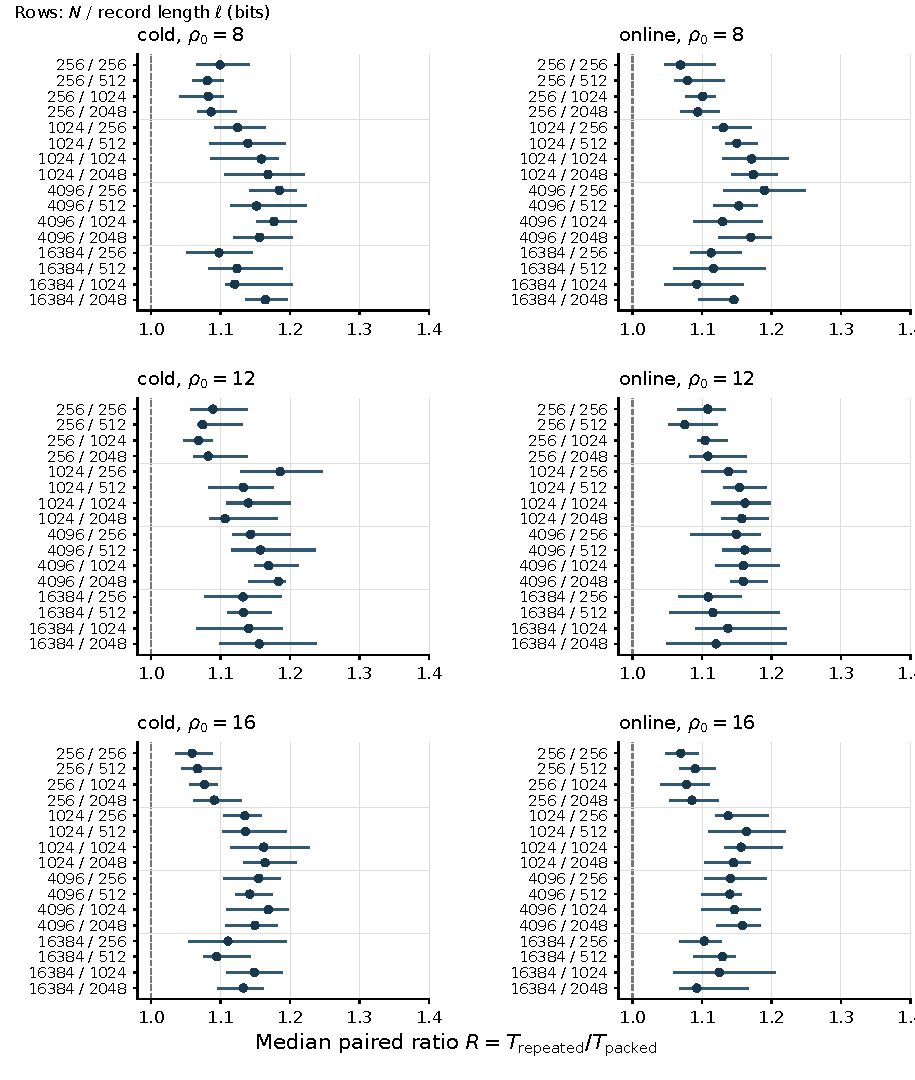
\includegraphics[width=\linewidth]{generated/primary.pdf}
\caption{Primary two-record comparison: all 96 cells. Points are median
paired repeated-to-packed task latency ratios; bars are pointwise 95\%
paired-bootstrap intervals. Cells remain separate; the figure makes no
family-wise or across-grid inference.}
\label{fig:primary-performance}
\end{figure}

\begin{table}[tbp]
\centering\small
\caption{Absolute task latency at the smallest and largest primary workload corners, with $\rho_0=8$. These four cells are descriptive examples; Fig.~\ref{fig:primary-performance} retains the full grid.}
\label{tab:absolute}
\setlength{\tabcolsep}{4pt}
\begin{tabular}{@{}rrlrrr@{}}
\toprule
$N$ & $\ell$ (bits) & View & Packed (s) & Repeated (s) & Paired $R$ \\
\midrule
256 & 256 & cold & 0.206 & 0.223 & 1.099 \\
256 & 256 & online & 0.169 & 0.180 & 1.069 \\
16384 & 2048 & cold & 14.315 & 16.743 & 1.164 \\
16384 & 2048 & online & 12.036 & 13.509 & 1.146 \\
\bottomrule\end{tabular}
\par\smallskip\begin{minipage}{\linewidth}\footnotesize Time columns are separate method medians. Their quotient is not the median paired ratio in the last column.\end{minipage}
\end{table}


\subsection{Multiplicity Experiment}
\label{sec:multiplicity}
The multiplicity experiment varies \(\alpha\in\{2,3,4\}\) at
\(N\in\{1024,4096\}\), \(\ell\in\{512,2048\}\), \(\rho_0=8\) and
\(w=8\alpha\), again with \(L=1\). Packed execution is a serial worker
pinned to one logical CPU. Repeated execution uses \(\alpha\) private
workers on distinct logical CPUs from a four-CPU set, which also bounds
the parent. Each worker has an 8 GiB address-space limit; aggregate
virtual memory has a separately sampled 16 GiB limit. Both width and
repeated-worker CPU count change with multiplicity. This is not a
fixed-total-core scaling comparison, and visible WSL core IDs do not
establish physical host isolation.

All 24 observed median ratios exceed one. Pointwise intervals exclude
one in all eight cells at each of \(\alpha=3,4\), but only three of eight
at \(\alpha=2\). All eight fixed-workload/view rows have
\(R_2<R_3<R_4\) (Table~\ref{tab:multiplicity}); this ordering is descriptive,
without a monotonicity significance test or universal scaling claim.

The two-record entries are internal references for this experiment.
All eight are smaller than their matched primary-experiment ratios, with
disjoint experiment-specific intervals. Extraction scope, API wrappers,
affinity, parent allowance, fixtures and sample schedules differ. In
particular, the primary adapter reads record-used fields, while the
multiplicity adapter extracts complete polynomial blocks with checked
wrappers. These differences have no established causal attribution. The
experiments remain separate; neither estimate is selected as the true
effect, and their samples are not pooled.
\begin{table}[tbp]
\centering\small
\caption{Multiplicity experiment at $\rho_0=8$, $w=8\alpha$ and $L=1$. Each cell contains ten measured pairs. Entries are median paired ratios with pointwise 95\% intervals.}
\label{tab:multiplicity}
\setlength{\tabcolsep}{4pt}
\begin{tabular}{@{}rrlccc@{}}
\toprule
$N$ & $\ell$ (bits) & View & $\alpha=2$ & $\alpha=3$ & $\alpha=4$ \\
\midrule
1024 & 512 & cold & \shortstack{1.050\\\scriptsize [1.005, 1.078]} & \shortstack{1.098\\\scriptsize [1.038, 1.129]} & \shortstack{1.140\\\scriptsize [1.119, 1.184]} \\[3pt]
1024 & 512 & online & \shortstack{1.055\\\scriptsize [1.030, 1.082]} & \shortstack{1.092\\\scriptsize [1.077, 1.107]} & \shortstack{1.151\\\scriptsize [1.106, 1.235]} \\[3pt]
1024 & 2048 & cold & \shortstack{1.036\\\scriptsize [1.006, 1.056]} & \shortstack{1.114\\\scriptsize [1.078, 1.137]} & \shortstack{1.154\\\scriptsize [1.117, 1.186]} \\[3pt]
1024 & 2048 & online & \shortstack{1.033\\\scriptsize [0.980, 1.067]} & \shortstack{1.096\\\scriptsize [1.074, 1.130]} & \shortstack{1.121\\\scriptsize [1.088, 1.143]} \\[3pt]
4096 & 512 & cold & \shortstack{1.025\\\scriptsize [1.000, 1.052]} & \shortstack{1.093\\\scriptsize [1.039, 1.106]} & \shortstack{1.122\\\scriptsize [1.095, 1.144]} \\[3pt]
4096 & 512 & online & \shortstack{1.024\\\scriptsize [0.998, 1.039]} & \shortstack{1.065\\\scriptsize [1.043, 1.083]} & \shortstack{1.108\\\scriptsize [1.094, 1.138]} \\[3pt]
4096 & 2048 & cold & \shortstack{1.013\\\scriptsize [0.986, 1.026]} & \shortstack{1.071\\\scriptsize [1.061, 1.080]} & \shortstack{1.129\\\scriptsize [1.110, 1.152]} \\[3pt]
4096 & 2048 & online & \shortstack{1.015\\\scriptsize [0.993, 1.034]} & \shortstack{1.066\\\scriptsize [1.053, 1.078]} & \shortstack{1.117\\\scriptsize [1.097, 1.158]} \\[3pt]
\bottomrule\end{tabular}
\par\smallskip\begin{minipage}{\linewidth}\footnotesize The two-record entries are internal references for this experiment. Packed execution is serial; repeated tasks use $\alpha$ concurrent workers. This is not a fixed-total-core comparison.\end{minipage}
\end{table}


\subsection{Bundle Sensitivity and Capacity}
\label{sec:capacity-evaluation}
The sensitivity experiment crosses two extraction/API bundles
(record-field and full-block) with the primary two-CPU and multiplicity
four-CPU-parent resource allowances. It holds \(N=1024\), \(\ell=512\),
\(\alpha=2\), \(\rho_0=8\) and the fixture generation rule fixed. Rebuilt
source variants retain their wrapper and extraction differences; resource
bundles include affinity and memory limits. A common runner records
monitor timestamps at a nominal 10 ms cadence; monitoring overhead has
not been shown to be zero. Extra record-field
coefficient validation occurs outside task timing. These are bundle
comparisons, not isolated changes to one operation.

The sensitivity and capacity designs were fixed before formal timing.
Each cell has three successive sessions, with three warmup and ten
measured pairs per session, balanced five/five method order and
interleaved cells. Cells do not execute concurrently, and pilot observations
are excluded. A failed or missing warmup
withholds that cell/session's latency summary; stopping rules retain
failed, incomplete and unstarted tasks and forbid effect-dependent sample
changes. All 702 scheduled pairs completed, including 540 measured pairs.
The reported intervals for these experiments are observed ranges of
three session medians, not confidence intervals or independent-day
replication.

Sensitivity median ratios range from 1.123 to 1.236. In each view and
implementation bundle, the descriptive median is larger under the
two-CPU resource allowance. The implementation ordering changes with
resource bundle and view. The two implementations' session ranges overlap
within each fixed resource bundle and view. The supplemental
table preserves all eight cells. These observations do not uniquely
explain the primary/multiplicity difference.

\paragraph{Two distinct capacity boundaries.}
Let \(u=\alpha J/n\). For \(L=1\), a coefficient-position representation
of the same fixed segments is
\[
 PM_{\rm position}(X)=\sum_{\nu=1}^{\alpha}
 X^{(\nu-1)J}P_{i_\nu}(X).
\]
It fits without overlapping coefficient ranges when \(\alpha J\le n\).
Radix packing uses coefficient values instead, subject to
\(t\ge B^\alpha\), no-wrap and native constraints. The quantity
\(\lceil\alpha J/n\rceil\) is a coefficient-slot lower bound, not the
reply count or runtime of an implemented alternative protocol. Other
encodings and hybrid schemes are not ruled out.

The boundary \(u=1\) differs from \(J=n\), where an individual record
starts to require more blocks. The capacity experiment fixes
\(N=1024\), \(\alpha=4\), \(\rho_0=8\), \(w=32\), full-block extraction
and the four-CPU parent allowance. Four lengths cross \(u=1\) while
retaining \(L=1\); a fifth has \(L=2\) (Table~\ref{tab:capacity}). All ten
median ratios exceed one, ranging from 1.258 to 1.339, without monotone
ordering in record length. These results establish finite capacity
coverage, not the speed of a coefficient-position comparator.
\begin{table}[tbp]
\centering\small
\caption{Capacity experiment: $N=1024$, $\alpha=4$, $\rho_0=8$, $w=32$, full-block extraction and the four-CPU parent allowance. Entries are median paired ratios with observed ranges of three session medians.}
\label{tab:capacity}
\setlength{\tabcolsep}{4pt}
\begin{tabular}{@{}rrrrcc@{}}
\toprule
$\ell$ (bits) & $J$ & $L$ & $u$ & Cold & Online \\
\midrule
4096 & 512 & 1 & 0.5 & 1.339 [1.312, 1.376] & 1.308 [1.232, 1.360] \\
8192 & 1024 & 1 & 1 & 1.311 [1.284, 1.318] & 1.271 [1.268, 1.286] \\
12288 & 1536 & 1 & 1.5 & 1.311 [1.277, 1.336] & 1.287 [1.287, 1.299] \\
16384 & 2048 & 1 & 2 & 1.319 [1.293, 1.337] & 1.258 [1.257, 1.266] \\
65536 & 8192 & 2 & 8 & 1.294 [1.275, 1.310] & 1.305 [1.293, 1.310] \\
\bottomrule\end{tabular}
\par\smallskip\begin{minipage}{\linewidth}\footnotesize Each cell has 30 measured pairs. Brackets are descriptive session ranges, not confidence intervals. Query buffers are 128/512 MiB for packed/repeated; reply buffers are 128/512 KiB for $L=1$ and 256/1024 KiB for $L=2$.\end{minipage}
\end{table}


\subsection{Payload and Resource Accounting}
For a declared ciphertext representation of size \(|C|\),
\begin{equation}\label{eq:payload}
 |Q|=N|C|,\qquad |\mathsf{Resp}|=L|C|.
\end{equation}
One native ciphertext occupies 131,072 bytes: two components, two RNS
limbs and 4096 64-bit words. Repeated retrieval copies \(\alpha N\)
query ciphertexts and \(\alpha L\) reply ciphertexts. These native
buffers are exactly \(\alpha\) times their packed counterparts, but
transport, framing, metadata and key distribution are unmeasured.
Canonical mathematical serialization can have a different size.

For byte-aligned records the raw database is \(N\ell/8\) bytes, counted
once regardless of multiplicity. The packed query remains larger than
this database at every reported length (Table~\ref{tab:payload}); even
at \(\ell=65536\) its ratio to raw size is 16. Thus same-profile buffer
savings do not establish raw-download or wire-traffic superiority.
\begin{table}[tbp]
\centering\small
\caption{Exact native buffer accounting for representative byte-aligned workloads with $\rho_0=8$. P/R denotes packed/repeated retrieval. Raw database size counts each record once.}
\label{tab:payload}
\setlength{\tabcolsep}{4pt}
\begin{tabular}{@{}rrrrcc@{}}
\toprule
$N$ & $\ell$ (bits) & $\alpha$ & Raw (KiB) & Query P/R (MiB) & Reply P/R (KiB) \\
\midrule
256 & 256 & 2 & 8 & 32/64 & 128/256 \\
16384 & 2048 & 2 & 4096 & 2048/4096 & 128/256 \\
1024 & 8192 & 4 & 1024 & 128/512 & 128/512 \\
1024 & 16384 & 4 & 2048 & 128/512 & 128/512 \\
1024 & 65536 & 4 & 8192 & 128/512 & 256/1024 \\
\bottomrule\end{tabular}
\par\smallskip\begin{minipage}{\linewidth}\footnotesize One ciphertext occupies 128 KiB. These are in-memory buffer sizes; transport, framing and metadata are unmeasured.\end{minipage}
\end{table}


Aggregate CPU work sums worker user-plus-system time, excluding parent
CPU. In the multiplicity experiment, repeated-to-packed ratios of
separate CPU medians are 1.972--2.052, 3.033--3.149 and 4.085--4.295 for
\(\alpha=2,3,4\). They describe work, not latency or a fitted scaling law.
Repeated RSS sums worker lifetime peaks, an upper bound rather than a
synchronized peak; online staging remains included and parent RSS is
separate. Phase sums likewise do not identify critical-path contributions.
Full summaries and machine-readable mappings accompany the supplement.
